\subsection{m-adic topologies on Noetherian rings}

PROPOSITION 4. Let A be a commutative Noetherian ring, m an ideal of A and E a finitely generated A-module. All the m-good filtrations on E define the same topology (namely the m-adic topology).

Let \((\mathbf{E}_{n})\) be an m-good filtration on E. As this filtration is exhaustive, every element of E belongs to one of the \(E_{n}\) and, as E is finitely generated and the \(E_{n}\) are A-modules, there exists an integer \(n_{1}\) such that \(E_{n_{1}} = E\) . On the other hand let \(n_{0}\) be such that \(mE_{n} = E_{n+1}\) for \(n \geqslant n_{0}\) ; then, for \(n > n_{0} - n_{1}\) , \(m^{n}E \subset E_{n+n_{1}} = m^{n+n_{1}-n_{0}}E_{n_{0}} \subset m^{n+n_{1}-n_{0}}E\) , which proves the proposition.

THEOREM 2 (Krull). Let A be a commutative Noetherian ring, m an ideal of A, E a finitely generated A-module and F a submodule of E. Then the m-adic topology on F is induced by the m-adic topology on E.

It follows from no. 1, Proposition 1 that the filtration induced on F by the m-adic filtration on E is m-good and the conclusion then follows from Proposition 4.

COROLLARY. Let A be a commutative Noetherian ring, m an ideal of A, E an A-module and F a finitely generated A-module. Every A-linear mapping u: E → F is a strict morphism (General Topology, Chapter III, § 2, no. 8) for the m-adic topologies.

As \(u(\mathfrak{m}^{n}\mathbf{E}) = \mathfrak{m}^{n}u(\mathbf{E})\) , u is a strict morphism of E onto \(u(\mathbf{E})\) for the m-adic topologies on these two modules and the m-adic topology on \(u(\mathbf{E})\) is induced by the m-adic topology on F by Theorem 2.

PROPOSITION 5. Let A be a commutative Noetherian ring, m an ideal of A and E a finitely generated A-module. The closure \(\bigcap_{n=1}^{\infty} \mathfrak{m}^{n}\mathrm{E}\) of \(\{0\}\) in E with respect to the m-adic topology is the set of \(x \in \mathrm{E}\) for which there exists an element \(m \in \mathfrak{m}\) such that \((1 - m)x = 0\) . If \(x = mx\) where \(m \in \mathfrak{m}\) , \(x = m^{n}x \in \mathfrak{m}^{n}\mathrm{E}\) for every integer \(n \geqslant 0\) and hence \(x \in \mathrm{F} = \bigcap_{n=0}^{\infty} \mathfrak{m}^{n}\mathrm{E}\) . Conversely, if \(x \in \mathrm{F}\) , Ax is contained in the intersection of the neighbourhoods of 0 in E; it then follows from Theorem 2 that the m-adic topology on Ax, which is induced by that on E, is the coarsest topology; as mx is by definition a neighbourhood of 0 with this topology, mx = Ax and hence there exists \(m \in \mathfrak{m}\) such that \(x = mx\) .

We may also say that mF = F since

\[
\mathrm{F} = \bigcap_ {n = 1} ^ {\infty} m ^ {n + 1} \mathrm{E} \subset m. \bigcap_ {n = 1} ^ {\infty} m ^ {n} \mathrm{E} = m \mathrm{F};
\]

as A is Noetherian, F is a finitely generated A-module; it is then sufficient to apply Chapter II, § 2, no. 2, Corollary 3 to Proposition 4.

COROLLARY (Krull). Let A be a commutative Noetherian ring and m an ideal of A. The ideal \(\bigcap_{n=1}^{\infty}m^{n}\) is the set of elements \(x\in A\) for which there exists \(m\in m\) such that \((1-m)x=0\) . In particular, for \(\bigcap_{n=1}^{\infty}m^{n}=\{0\}\) , it is necessary and sufficient that no element of \(1+m\) be a divisor of 0 in A.

It is sufficient to apply Proposition 5 to \(\mathbf{E} = \mathbf{A}_s\) .

\pandocbounded{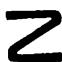
\includegraphics[keepaspectratio]{images/part002_69a966b6.jpg}}

Remark. The hypothesis that A is Noetherian is essential in this corollary. For example, let A be the ring of infinitely differentiable mappings from R to itself and let m be the (maximal) ideal of A consisting of the functions f such that \(f(0) = 0\) . It is immediate that \(\bigcap_{n=0}^{\infty} m^{n}\) is the set of functions f such that

\(f^{(n)}(0) = 0\) for all \(n \geqslant 0\) and there exist such functions with \(f(x) \neq 0\) , for all \(x \neq 0\) , for example the function \(f\) defined by \(f(x) = e^{-1 / x^2}\) for \(x \neq 0\) and \(f(0) = 0\) .

DEFINITION 1. Let A be a topological ring. If a two-sided ideal m of A is such that the given topology on A is the m-adic topology, m is called a defining ideal of the topology on A.

Let A be a commutative Noetherian ring, m an ideal of A and t its radical (Chapter II, § 2, no. 6). If \(m'\) is a defining ideal of the m-adic topology, there exists an integer n \textgreater{} 0 such that \(m'^{n} \subset m\) (§ 2, no. 5) and hence \(m' \subset t\) ; conversely, since A is Noetherian, there exists an integer k \textgreater{} 0 such that \(t^{k} \subset m\) (Chapter II, § 2, no. 6, Proposition 15) and hence t is the largest defining ideal of the m-adic topology.

